\documentclass[a4paper,12pt]{article}
\usepackage[ukrainian,english]{babel}
\usepackage{ucs}
\usepackage[utf8]{inputenc}
\usepackage[T2A]{fontenc}
\usepackage{amsmath}
\usepackage{amsfonts}
\usepackage{graphicx}
\usepackage{wrapfig}
\usepackage{multirow}
\usepackage{flafter}
\usepackage{lscape}
\usepackage{booktabs}
\newcommand\tab[1][1cm]{\hspace*{#1}}
\usepackage[left=20mm, top=20mm, right=10mm, bottom=20mm, nohead, nofoot]{geometry}
\begin{document}
\begin{center}
\begin{titlepage}
   \begin{center}
       \vspace*{1cm}



       \vspace{0.5cm}
        {\LARGE Лабораторна робота №1}
            
       \vspace{1.5cm}

       \textbf{Бекешева Анастасія ФІ-12}

       \vfill
            
       \vspace{0.8cm}
            
       22.02.2022
            
   \end{center}
\end{titlepage}

\tableofcontents
\newpage 
\end{center}
\section{Заголовок}
\begin{enumerate}
	\item \emph{Назва роботи:} \\\indent Вивчення прямолінійного руху тіл у полі тяжіння за допомогою машини Атвуда
	\item \emph{Мета роботи:}\\ \indent Визначити прискорення вільного падіння в полі тяжіння Землі за допомогою машини Атвуда.
	\item \emph{Теоретична довідка:}\\  \indent Машину Атвуда було створено для вичення закону руху тіл у полі сили тяжіння. Прискорення земного тяжіння занадто велике, тому вивчати його краще на дуже високому приладі, або за допомогою точних годинників. Але машина Атвуда дозволяє сповільнити рух тіл до зручних для вимірювання швидкостей, щоб за допомогою звичайних приладів визначити прискорення вільного падіння. \\
	\indent Сила тяжіння  - сили яка діє на будь-яке тіло, що знаходиться поблизу поверхні Землі або іншого астрономічного тіла. Вона надає всім тілам будь-якої маси однакового прискорення.\\
	\indent  Рівномірний прямолінійний рух -  рух, під час якого тіло за будь-які однакові проміжки часу здійснює однаковеі переміщення. \\
	 \indent Прискорення - векторна фізична величина, похідна швидкості по часу і за величиною дорівнює зміни швидкості тіла за одиницю часу. \\
	 \indent Рівноприскорений рух - це рух, під час якого швидкість руху тіла за будь-які рівні інтервали часу змінюється однаково. \\
	 

\end{enumerate}
\section{Визначення законів руху для тягарців}$\\$
\indent Для визначення закону руху тягарця виберемо нерухому систему відліку з центром на осі блоку Вісь Х спрямовано вертикально вниз. \\
\indent На тягарець а діє сила тяжіння $M+\frac mg$ та сила натягу нитки $T$. Тому за другим законом Ньютона:
\begin{equation}\label{Newton1}
	(M+m)g-T_1=(M+m)a,\tab a\textrm{ - прискорення тягарця}
\end{equation}
\indent Другий закон Ньютона для другуго тягарця:
\begin{equation}\label{Newton2}
	Mg-T_2=-Ma
\end{equation}
\indent Співвідношення між силами натягу(якщо знехтувати тертям):
\begin{equation}
	(T_1-T_2)r=\frac{Ja}{r},\tab J \textrm{ - момент інерції},\>r\textrm{ - радіус}
\end{equation}
\indent З рівнянь дістаємо зв'язок між прискоренням та прискоренням тягарців:
\begin{equation}
	a=g\frac{m}{2M+m+\frac{J}{r^2}}
\end{equation}
\indent Формула спрощується, якщо застосувати момент інерції:
\begin{equation}\label{a_theor}
	a=g\frac{m}{2m+M}
\end{equation}\newpage	
\indent Тягарець набуває швидкості між кронштейнами 2 і 3:\\
	$v=\sqrt{2h_1a},\>h_1\textrm{ - відстань між кронштейнами }\Rightarrow v=\frac{h_2}{t},\>h_2 \textrm{ - відстань між кронштейнами 3 i 4},\\\>t\textrm{ - час руху між ними .}$
\indent Звідси: 
\begin{equation}\label{a_exp}
	a=\frac{h_2^2}{2h_1t}
\end{equation}
\indent Тоді отримуємо формулу для визначення $g$:
\begin{equation}
	g=\frac{(2M+m)h_2^2}{2mh_1t}
\end{equation}
\section{Опис експерементальної роботи}
\begin{wrapfigure}{L}{5cm}
\centering
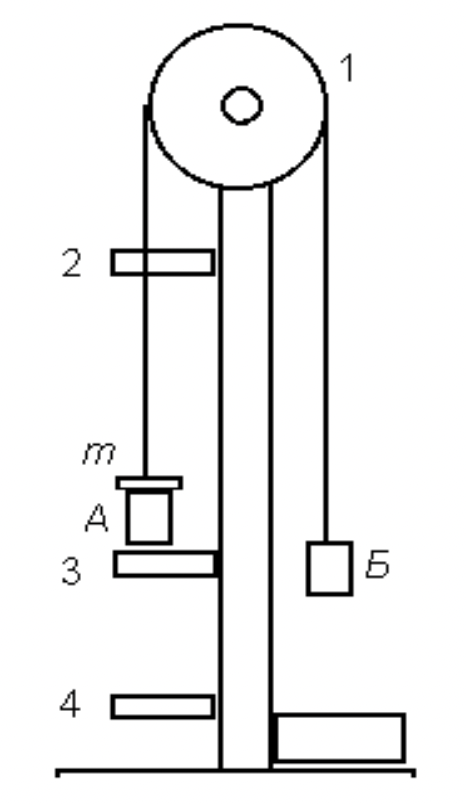
\includegraphics[height=5.5cm]{atwood.png}
\end{wrapfigure}
\indent \indent На рисунку зображено машину Атвуда.\\ \indent Через лекий блок, який вільно обертається перекінуто нитку, на кінцях якоЇ висять тягарці А і Б. Якщо на тягарець покласти вантаж, то рівновагу буде порушено, і система почне рухатись з прискоренням. На колоні закріплено кронштейни 2, 3, 4. Кронштейн 2 фіксує початкові положення тягарця А, а на 3, 4 розміщенні фотодатчики.\\\indent На початку експеременту тягарець зафіксовано. Далі він починає рухатись. Потім на рівні з кронштейном додатковий вантаж знімається, і система з 2 вантажів починає рухатись рівномірно. Фотодатчики фіксують час рівномірного руху тягарця.\\
\section{Хід роботи}
\subsection{Хід експеременту.} $\\$
\indent Час руху вимірюється електронним секундоміром, який вмиккається та вимикається при проходженні тягарцем оптичної осі фотодатчиків 3 та 4, відповідно. При натисканні конпки 'Пуск' вимикаются гальмо, яке утримує тягарець в початковому положені, секундомір приходить у етап очікування і запускається при проходженні тягарцем фотодатчика 3. Після проходження фотодатчика 4 секундомір вимикається гальмо. \\
\indent Висота падіння визначається за шкалою, що наневена на стояк, за різницею положень оптичних осей верхнього та нижнього фотодатчика. Маса кожного тягарця визначається експерементально. Похибка кронштейнів 2, 3, 4 є $\pm 1$ мм. Похибка по часу - 0,001 с.\\
\subsection{Хід обчислювань. }
	\begin{enumerate}
		\item Визначимо прискорення системи тягарців з вантажами. Фіксуємо кронштейном 3. Проводимо серію з 10 експерементів.
		\item Проводимо експеремнти для всіх наявних вантажів та їх різних комбінацій.
		\item Міняємо положення 3 і повторюємо дослід.
		\item Зважуємо тягарці $M$ та $m$. Оцінюємо із наших даних значення $g$. 
	\end{enumerate}
\subsection{Етапи обробки результатів експеременту}
\begin{enumerate}
	\item Усереднюємо час $t$ для кожного експеременту з окремими вантажем $m$ та фіксованими $h_1$ і $h_2$. Визначаємо випадкову похибку часу та порівнюємо із похибкою, яку вносить секундомір. 
	\item Для кожного випадку, розраховуємо $a$ i $g$. Визначаємо похибки.
	\item Будуємо графік залежності $g$ від $\frac1m$
	\item Оцінюємо похибку експеременту.
\end{enumerate}
\newpage
\section{Експерементальні дані}
\begin{table}[htp]
\begin{tabular}{@{}|l|l|l|l|l|l|l|l|l|l|@{}}
\toprule
t     & \textless{}t\textgreater{} & $\delta(t)$               & $<\delta(t)>$              & M                      & m                      & $h_1$                 & $h_2$                 & \multicolumn{1}{l}{$a_{exp}$}                 & $a_{theor}$                                   \\ \midrule
1,234 & \multirow{3}{*}{1,241}     & \multirow{3}{*}{0,008337} & \multirow{27}{*}{0,013676} & \multirow{3}{*}{0,062} & \multirow{3}{*}{0,006} & \multirow{3}{*}{0,11} & \multirow{3}{*}{0,34} & \multirow{3}{*}{0,341186}                     & \multirow{3}{*}{0,452792}                     \\
1,25  &                            &                           &                            &                        &                        &                       &                       &                                               &                                               \\
1,238 &                            &                           &                            &                        &                        &                       &                       &                                               &                                               \\\hline
t     & \textless{}t\textgreater{} & $\delta(t)$               &                            & M                      & m                      & $h_1$                 & $h_2$                 & \multicolumn{1}{l}{$a_{exp}$}                 & $a_{theor}$                                   \\\hline
1,062 & \multirow{3}{*}{1,084}     & \multirow{3}{*}{0,023032} &                            & \multirow{3}{*}{0,062} & \multirow{3}{*}{0,008} & \multirow{3}{*}{0,11} & \multirow{3}{*}{0,34} & \multirow{3}{*}{0,447174}                     & \multicolumn{1}{r}{\multirow{3}{*}{0,594576}} \\
1,108 &                            &                           &                            &                        &                        &                       &                       &                                               & \multicolumn{1}{r}{}                          \\
1,083 &                            &                           &                            &                        &                        &                       &                       &                                               & \multicolumn{1}{r}{}                          \\\hline
t     & \textless{}t\textgreater{} & $\delta(t)$               &                            & M                      & m                      & $h_1$                 & $h_2$                 & \multicolumn{1}{l}{$a_{exp}$}                 & $a_{theor}$                                   \\\hline
0,97  & \multirow{3}{*}{0,964}     & \multirow{3}{*}{0,012165} &                            & \multirow{3}{*}{0,062} & \multirow{3}{*}{0,01}  & \multirow{3}{*}{0,11} & \multirow{3}{*}{0,34} & \multirow{3}{*}{0,565433}                     & \multicolumn{1}{r}{\multirow{3}{*}{0,732127}} \\
0,95  &                            &                           &                            &                        &                        &                       &                       &                                               & \multicolumn{1}{r}{}                          \\
0,972 &                            &                           &                            &                        &                        &                       &                       &                                               & \multicolumn{1}{r}{}                          \\\hline
t     & \textless{}t\textgreater{} & $\delta(t)$               &                            & M                      & m                      & $h_1$                 & $h_2$                 & \multicolumn{1}{l}{$a_{exp}$}                 & $a_{theor}$                                   \\\hline
0,756 & \multirow{3}{*}{0,771}     & \multirow{3}{*}{0,001581} &                            & \multirow{3}{*}{0,062} & \multirow{3}{*}{0,014} & \multirow{3}{*}{0,11} & \multirow{3}{*}{0,34} & \multirow{3}{*}{0,883947}                     & \multirow{3}{*}{0,995268}                     \\
0,788 &                            &                           &                            &                        &                        &                       &                       &                                               &                                               \\
0,769 &                            &                           &                            &                        &                        &                       &                       &                                               &                                               \\\hline
t     & \textless{}t\textgreater{} & $\delta(t)$               &                            & M                      & m                      & $h_1$                 & $h_2$                 & \multicolumn{1}{l}{$a_{exp}$}                 & $a_{theor}$                                   \\\hline
0,698 & \multirow{3}{*}{0,699}     & \multirow{3}{*}{0,001581} &                            & \multirow{3}{*}{0,062} & \multirow{3}{*}{0,016} & \multirow{3}{*}{0,11} & \multirow{3}{*}{0,34} & \multicolumn{1}{l}{\multirow{3}{*}{1,075427}} & \multirow{3}{*}{1,1212}                       \\
0,699 &                            &                           &                            &                        &                        &                       &                       & \multicolumn{1}{l}{}                          &                                               \\
0,701 &                            &                           &                            &                        &                        &                       &                       & \multicolumn{1}{l}{}                          &                                               \\\hline
t     & \textless{}t\textgreater{} & $\delta(t)$               &                            & M                      & m                      & $h_1$                 & $h_2$                 & \multicolumn{1}{l}{$a_{exp}$}                 & $a_{theor}$                                   \\\hline
0,707 & \multirow{3}{*}{0,688}     & \multirow{3}{*}{0,021829} &                            & \multirow{3}{*}{0,062} & \multirow{3}{*}{0,018} & \multirow{3}{*}{0,11} & \multirow{3}{*}{0,34} & \multicolumn{1}{l}{\multirow{3}{*}{1,11009}}  & \multicolumn{1}{r}{\multirow{3}{*}{1,243584}} \\
0,664 &                            &                           &                            &                        &                        &                       &                       & \multicolumn{1}{l}{}                          & \multicolumn{1}{r}{}                          \\
0,692 &                            &                           &                            &                        &                        &                       &                       & \multicolumn{1}{l}{}                          & \multicolumn{1}{r}{}                          \\\hline
t     & \textless{}t\textgreater{} & $\delta(t)$               &                            & M                      & m                      & $h_1$                 & $h_2$                 & \multicolumn{1}{l}{$a_{exp}$}                 & $a_{theor}$                                   \\\hline
0,596 & \multirow{3}{*}{0,582}     & \multirow{3}{*}{0,012767} &                            & \multirow{3}{*}{0,062} & \multirow{3}{*}{0,024} & \multirow{3}{*}{0,11} & \multirow{3}{*}{0,34} & \multirow{3}{*}{1,551276}                     & \multirow{3}{*}{1,590892}                     \\
0,579 &                            &                           &                            &                        &                        &                       &                       &                                               &                                               \\
0,571 &                            &                           &                            &                        &                        &                       &                       &                                               &                                               \\ \hline
\end{tabular}
\end{table}
% Please add the following required packages to your document preamble:
% \usepackage{booktabs}
% \usepackage{multirow}
\begin{table}[]
\begin{tabular}{@{}|c|l|l|l|l|l|@{}}
\toprule
\multicolumn{1}{l}{rel $\delta(a)$}          & rel $<\delta(a)>$          & $g_{pr}$                                      & $g_{theor}$              & rel $\delta(g)$                               & rel $<\delta(g)>$      \\ \midrule
\multirow{3}{*}{0,327112}                    & \multirow{27}{*}{0,180834} & \multicolumn{1}{r}{\multirow{3}{*}{7,392363}} & \multirow{27}{*}{9,8105} & \multicolumn{1}{c}{\multirow{3}{*}{0,327113}} & \multirow{27}{*}{14\%} \\
                                             &                            & \multicolumn{1}{r}{}                          &                          & \multicolumn{1}{c}{}                          &                        \\
                                             &                            & \multicolumn{1}{r}{}                          &                          & \multicolumn{1}{c}{}                          &                        \\\hline
\multicolumn{1}{l}{rel $\delta(a)$}          &                            & $g_{pr}$                                      &                          & rel $\delta(g)$                               &                        \\
\multicolumn{1}{r}{\multirow{3}{*}{0,32963}} &                            & \multicolumn{1}{r}{\multirow{3}{*}{7,378371}} &                          & \multirow{3}{*}{0,329629}                     &                        \\\hline
\multicolumn{1}{r}{}                         &                            & \multicolumn{1}{r}{}                          &                          &                                               &                        \\
\multicolumn{1}{r}{}                         &                            & \multicolumn{1}{r}{}                          &                          &                                               &                        \\\hline
\multicolumn{1}{l}{rel $\delta(a)$}          &                            & $g_{pr}$                                      &                          & rel $\delta(g)$                               &                        \\
\multirow{3}{*}{0,294808}                    &                            & \multirow{3}{*}{7,576802}                     &                          & \multicolumn{1}{c}{\multirow{3}{*}{0,294807}} &                        \\\hline
                                             &                            &                                               &                          & \multicolumn{1}{c}{}                          &                        \\
                                             &                            &                                               &                          & \multicolumn{1}{c}{}                          &                        \\\hline
\multicolumn{1}{l}{rel $\delta(a)$}          &                            & $g_{pr}$                                      &                          & rel $\delta(g)$                               &                        \\
\multirow{3}{*}{0,125936}                    &                            & \multirow{3}{*}{8,713192}                     &                          & \multicolumn{1}{c}{\multirow{3}{*}{0,125936}} &                        \\\hline
                                             &                            &                                               &                          & \multicolumn{1}{c}{}                          &                        \\
                                             &                            &                                               &                          & \multicolumn{1}{c}{}                          &                        \\\hline
\multicolumn{1}{l}{rel $\delta(a)$}          &                            & $g_{pr}$                                      &                          & rel $\delta(g)$                               &                        \\
\multirow{3}{*}{0,042563}                    &                            & \multicolumn{1}{r}{\multirow{3}{*}{9,409986}} &                          & \multirow{3}{*}{0,042563}                     &                        \\\hline
                                             &                            & \multicolumn{1}{r}{}                          &                          &                                               &                        \\
                                             &                            & \multicolumn{1}{r}{}                          &                          &                                               &                        \\\hline
\multicolumn{1}{l}{rel $\delta(a)$}          &                            & $g_{pr}$                                      &                          & rel $\delta(g)$                               &                        \\
\multirow{3}{*}{0,120255}                    &                            & \multicolumn{1}{r}{\multirow{3}{*}{8,757377}} &                          & \multirow{3}{*}{0,120255}                     &                        \\\hline
                                             &                            & \multicolumn{1}{r}{}                          &                          &                                               &                        \\
                                             &                            & \multicolumn{1}{r}{}                          &                          &                                               &                        \\\hline
\multicolumn{1}{l}{rel $\delta(a)$}          &                            & $g_{pr}$                                      &                          & rel $\delta(g)$                               &                        \\
\multirow{3}{*}{0,025538}                    &                            & \multirow{3}{*}{9,566202}                     &                          & \multicolumn{1}{c}{\multirow{3}{*}{0,025538}} &                        \\\hline
                                             &                            &                                               &                          & \multicolumn{1}{c}{}                          &                        \\
                                             &                            &                                               &                          & \multicolumn{1}{c}{}                          &\\                       
\hline
\end{tabular}
\end{table}
\newpage
 \section{Обробка результатів експеременту}$\\$
\indent Результати дослідів оформлені у вигляді таблиць. \\
\indent $<t>$ - середній час для кожної маси перевантаження.
За формулою (\ref{a_exp}), $a_{exp}=\frac{h_2^2}{2h_1t}$,\\ де $h_1=0,11m,\>h_2=0,34m$ визначили експериментальне значення прискорення тягарця. \\
\indent Теоретичне значення прискорення тягарця визначали за формулою (\ref{a_theor}): $a_{theor}=\frac{gm}{2M+m}$,\\ де $g=g_{theor},\> M$ - маса тягарця, $m$ - маса вантажка, який поклали на тягарець. \\
\indent Прискорення вільного падіння знаходили так(\ref{a_theor}): $g=\frac{a_{exp}(2M+m)}{m}$.\\
\indent Для розрахунку похибок використовували такі формули:\\
Aбсолютна похибка прискорення вільного падіння: rel$\delta(g)=g_{theor}-<g_{pr}>$\\
Bідносна похибка прискорення вільного падіння: rel$<\delta(g)>=\frac{g_{theor}-g_{pr}}{g_{theor}}\cdot 100\%$\\
Bідносна похибка прискорення $a$: rel$<\delta(a)>=\frac{a_{theor}-a_{exp}}{a_{exp}}\cdot 100\%$\\
Bипадкова похибка за часом: $<\delta(t)>=\sqrt{\frac{1}{n-1}\sum\limits_{i=1}^{n}(t_i-<t>)^2}$, \\де $n$ - кількість вимірювань часу $t$\\
\emph{Висновок:}\\ Bизначила прискорення вільного падіння в полі тяжіння Землі за допомогою машини Атвуда.
\section{Графік}\begin{center}
	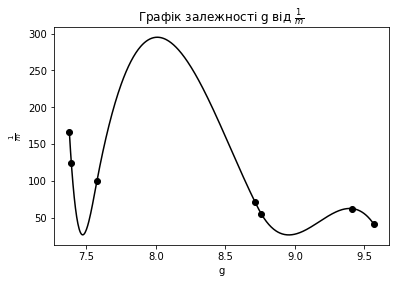
\includegraphics{graph2.png}
\end{center}


\end{document}